\documentclass[11pt,a4paper,oneside]{report}             % Single-side

%\PassOptionsToPackage{chapternumber=Huordinal}{magyar.ldf}
\usepackage{t1enc}
\usepackage[utf8]{inputenc}
\usepackage{amsmath}
\usepackage{amssymb}
\usepackage{enumerate}
\usepackage[amsmath,thmmarks]{ntheorem}
\usepackage{graphics}
\usepackage{epsfig}
\usepackage{listings}
\usepackage{color}
%\usepackage{fancyhdr}
\usepackage{lastpage}
\usepackage{anysize}
\usepackage[english]{babel}
\usepackage{sectsty}
\usepackage{setspace}  % Ettol a tablazatok, abrak, labjegyzetek maradnak 1-es sorkozzel!
\usepackage[hang]{caption}
\usepackage{hyperref}
\usepackage[final]{pdfpages}
%\usepackage{minted}
\usepackage{lscape}
\usepackage{float}
\usepackage{subcaption}
\usepackage{csquotes}

%--------------------------------------------------------------------------------------
% Main variables
%--------------------------------------------------------------------------------------
\newcommand{\vikszerzo}{Dávid Danyi}
\newcommand{\vikkonzulens}{Viktor Kovács}
\newcommand{\vikcim}{Marker Based Localisation and Pose Estimation Using Image Processing}
\newcommand{\viktanszek}{Department of Automation and Applied Informatics}
\newcommand{\vikdoktipus}{Thesis}
\newcommand{\vikdepartmentr}{Dávid Danyi}

%--------------------------------------------------------------------------------------
% Page layout setup
%--------------------------------------------------------------------------------------
% we need to redefine the pagestyle plain
% another possibility is to use the body of this command without \fancypagestyle
% and use \pagestyle{fancy} but in that case the special pages
% (like the ToC, the References, and the Chapter pages)remain in plane style

\pagestyle{plain}
\setlength{\parindent}{0pt} % áttekinthetőbb, angol nyelvű dokumentumokban jellemző
\setlength{\parskip}{8pt plus 3pt minus 3pt} % áttekinthetőbb, angol nyelvű dokumentumokban jellemző
%\setlength{\parindent}{12pt} % magyar nyelvű dokumentumokban jellemző
%\setlength{\parskip}{0pt}    % magyar nyelvű dokumentumokban jellemző

\marginsize{35mm}{25mm}{15mm}{15mm} % anysize package
\setcounter{secnumdepth}{0}
\sectionfont{\large\upshape\bfseries}
\setcounter{secnumdepth}{2}
\singlespacing
\frenchspacing

%--------------------------------------------------------------------------------------
%	Setup hyperref package
%--------------------------------------------------------------------------------------
\hypersetup{
    bookmarks=true,            % show bookmarks bar?
    unicode=false,             % non-Latin characters in Acrobat’s bookmarks
    pdftitle={\vikcim},        % title
    pdfauthor={\vikszerzo},    % author
    pdfsubject={\vikdoktipus}, % subject of the document
    pdfcreator={\vikszerzo},   % creator of the document
    pdfproducer={Producer},    % producer of the document
    pdfkeywords={keywords},    % list of keywords
    pdfnewwindow=true,         % links in new window
    colorlinks=true,           % false: boxed links; true: colored links
    linkcolor=black,           % color of internal links
    citecolor=black,           % color of links to bibliography
    filecolor=black,           % color of file links
    urlcolor=black             % color of external links
}

%--------------------------------------------------------------------------------------
% Set up listings
%--------------------------------------------------------------------------------------
\lstset{
	basicstyle=\scriptsize\ttfamily, % print whole listing small
	keywordstyle=\color{black}\bfseries\underbar, % underlined bold black keywords
	identifierstyle=, 					% nothing happens
	commentstyle=\color{white}, % white comments
	stringstyle=\scriptsize\sffamily, 			% typewriter type for strings
	showstringspaces=false,     % no special string spaces
	aboveskip=3pt,
	belowskip=3pt,
	columns=fixed,
	backgroundcolor=\color{lightgray},
} 		
\def\lstlistingname{listing}

%--------------------------------------------------------------------------------------
% Set up minted
%--------------------------------------------------------------------------------------	
%\definecolor{bg}{rgb}{0.95,0.95,0.95}
%\usemintedstyle{emacs}

%--------------------------------------------------------------------------------------
%	Some new commands and declarations
%--------------------------------------------------------------------------------------
\newcommand{\code}[1]{{\upshape\ttfamily\scriptsize\indent #1}}

% define references
\newcommand{\figref}[1]{\ref{fig:#1}.}
\renewcommand{\eqref}[1]{(\ref{eq:#1})}
\newcommand{\listref}[1]{\ref{listing:#1}.}
\newcommand{\sectref}[1]{\ref{sect:#1}}
\newcommand{\tabref}[1]{\ref{tab:#1}.}

\DeclareMathOperator*{\argmax}{arg\,max}
%\DeclareMathOperator*[1]{\floor}{arg\,max}
\DeclareMathOperator{\sign}{sgn}
\DeclareMathOperator{\rot}{rot}
\definecolor{lightgray}{rgb}{0.95,0.95,0.95}

\author{\vikszerzo}
\title{\viktitle}
\includeonly{
	titlepage,%
	declaration,%
	abstract,%
	abbreviations,%
	introduction,%
	pose, %
	marker,%
	quad_detection,%
	marker_recognition, %
	%chapter3,%
	%conclusion, %
	%appendices,%
}

%--------------------------------------------------------------------------------------
%	Setup captions
%--------------------------------------------------------------------------------------
\captionsetup[figure]{
%labelsep=none,
%font={footnotesize,it},
%justification=justified,
width=.75\textwidth,
aboveskip=10pt}

\renewcommand{\captionlabelfont}{\small\bf}
\renewcommand{\captionfont}{\footnotesize\it}

%--------------------------------------------------------------------------------------
% Table of contents and the main text
%--------------------------------------------------------------------------------------
\begin{document}

\includepdf{feladatkiiras.pdf}
\pagenumbering{arabic}
\onehalfspacing
%--------------------------------------------------------------------------------------
%	The title page
%--------------------------------------------------------------------------------------
\begin{titlepage}
\begin{center}

\includegraphics[width=60mm,keepaspectratio]{figures/BMElogo.png}\\
\vspace{0.3cm}
\textbf{Budapest University of Technology and Economics}\\
\textmd{Faculty of Electrical Engineering and Informatics}\\
\textmd{\viktanszek}\\[5cm]

\vspace{0.4cm}
{\huge \bfseries \vikcim}\\[0.8cm]
\vspace{0.5cm}
\textsc{\Large \vikdoktipus}\\[4cm]

\begin{tabular}{cc}
 \makebox[7cm]{\emph{Author}} & \makebox[7cm]{\emph{Consultant}} \\
 \makebox[7cm]{\vikszerzo} & \makebox[7cm]{\vikkonzulens}
\end{tabular}

\vfill
{\large \today}
\end{center}
\end{titlepage}
\tableofcontents\vfill
%--------------------------------------------------------------------------------------
% Nyilatkozat
%--------------------------------------------------------------------------------------
\begin{center}
\large
\textbf{HALLGATÓI NYILATKOZAT}\\
\end{center}

Alulírott \emph{\vikszerzo}, szigorló hallgató kijelentem, hogy ezt a szakdolgozatot meg nem engedett segítség nélkül, saját magam készítettem, csak a megadott forrásokat (szakirodalom, eszközök stb.) használtam fel. Minden olyan részt, melyet szó szerint, vagy azonos értelemben, de átfogalmazva más forrásból átvettem, egyértelmûen, a forrás megadásával megjelöltem.

Hozzájárulok, hogy a jelen munkám alapadatait (szerzõ(k), cím, angol és magyar nyelvû tartalmi kivonat, készítés éve, konzulens(ek) neve) a BME VIK nyilvánosan hozzáférhetõ elektronikus formában, a munka teljes szövegét pedig az egyetem belsõ hálózatán keresztül (vagy autentikált felhasználók számára) közzétegye. Kijelentem, hogy a benyújtott munka és annak elektronikus verziója megegyezik. Dékáni engedéllyel titkosított diplomatervek esetén a dolgozat szövege csak 3 év eltelte után válik hozzáférhetõvé.

\begin{flushleft}
\vspace*{1cm}
Budapest, \today
\end{flushleft}

\begin{flushright}
 \vspace*{1cm}
 \makebox[7cm]{\rule{6cm}{.4pt}}\\
 \makebox[7cm]{\emph{\vikszerzo}}\\
 \makebox[7cm]{hallgató}
\end{flushright}
\thispagestyle{empty}

\vfill
\clearpage
\thispagestyle{empty} % an empty page


%----------------------------------------------------------------------------
% Abstract in hungarian
%----------------------------------------------------------------------------
\chapter*{Kivonat}\addcontentsline{toc}{chapter}{Kivonat}
A képfeldolgozás nem újkeletű tudományterület, már évtizedek óta folynak kutatások ezen a téren.
Sok, ma is használt algoritmust az 1960-as években fejlesztettek ki.
Akkoriban főleg a tudósok körében használt, drága eszköznek számított a számítógépes képfeldolgozás.
Műholdképek, orvosdiagnosztikai adatok elemzésére, optikai karakterfelismerésre használták.
Az olcsó és nagy teljesítményű, általános felhasználású számítógépek terjedésével azonban új lehetőségek nyíltak meg ezen a területen.
Lehetővé vált például a valósidejű képfeldolgozó algoritmusok futtatása.
Ezen fejlődés nélkül lehetetlen lett volna a 3 dimenziós látórendszerek kifejlesztése.
Ezek a rendszerek jóval számításigényesebbek a klasszikus képfeldolgozási problémáknál, de a mai technológiával már ezek a megoldások és elérhetőek az átlagos felhasználók számára.
Ennek legfőbb jele a robot navigációs, virtuális- és kiterjesztett valóság alkalmazások széleskörű megjelenése.

Jelen munka a fiduciális markerek alapján történő nézőpont meghatározás alkalmazhatóságát vizsgálja.
A nézőpont-meghatározás célja a kamera pozíciójának és orientációjának meghatározása egy ismert markerhez viszonyítva.
Ez egy összetett feladat aminek a megoldása több képfeldolgozási- és optimalizációs feladat megoldását igényli.
Ez a dolgozat be fogja mutatni a kép alapján történő nézőpont-meghatározás lépéseit.

A munka első részében ismertetésre kerül a nézőpont-meghatározási probléma.
Először röviden össze lesz foglalva a P-n-P néven ismert probléma: a nézőpont meghatározás $n$ pontpár alapján, aminek ismert a világkoordinátákban adott helyzete, valamint a képi helyzetük is.
Ezt a problémát többen többféleképp megoldották, néhány ilyen megoldás alapvető gondolatmenete összefoglalásra kerül.
Ennek a szakasznak a zárásaként összehasonlítom az eljárásokat és kiválasztom a tulajdonságaik alapján a projekt céljára a legideálisabbat.

A pozicionálás pontosságát és robusztusságát nagyban befolyásolhatja az alkalmazott fiduciális marker is.
Vannak ugyan már elterjedt markertípusok (ARTag, glyph, stb...), de jelen munkában kísérletet teszek egy új marker tervezésére.
Ez az új marker megpróbál jobb eredményt nyújtani bizonyos területek, mint a már elterjedt megoldások.
Ezen marker alkalmazhatósága is vizsgálva lesz ebben a dolgozatban.

A dolgozat utolsó nagyobb része a markerek felismerésére használt képfeldolgozási eljárásokról fog szólni.
A különböző algoritmusok rövid elméleti áttekintése után egy-egy implementációs javaslat is közlésre kerül.
A felismerő eljárások hatékonysága is vizsgálat alá kerül, ideális és zajos képeken egyaránt.
A mérési eredmények alapján javasolni fogok egy, a projekt számára optimális markerfelismerő eljárást.
\vfill

%----------------------------------------------------------------------------
% Abstract in english
%----------------------------------------------------------------------------
\chapter*{Abstract}\addcontentsline{toc}{chapter}{Abstract}
Image processing has been an intensively researched subject for decades.
Many algorithms that are used today have been developed in the 1960s.
At that time, it was a costly tool mainly used by scientists for satellite imagery, medical imaging, optical character recognition, etc...
The advancement of cheap and powerful general purpose computers opened up new possibilities for research and application.
Real time image processing became possible.
An interesting and even more computationally expensive sub-field of computer vision is 3D reconstruction.
With today's (consumer) technology it is possible to map the 3D world based on image processing solutions.
Navigational, Augmented and Virtual Reality applications are spreading.

This paper will examine the use of fiducial markers for camera pose estimation using a single camera.
The goal of pose estimation is to determine the position and orientation of the camera with respect to a known marker.
This is a complex task, which involves multiple image processing steps, as well as solving optimization problems.
This work will provide an overview of the steps necessary for estimating the camera pose based on picture of a fiducial marker.

A section of this work will be dedicated to the pose estimation problem.
There will be a short summary of the problem of reconstructing the view point based on point pairs in the world coordinate system and image points.
Then some algorithms will be summarised that solved that problem.
This section will be closed by comparing the benefits and drawbacks of these algorithms and choosing the one that best suits the need of this project.

The choice of the marker also influences accuracy and robustness of the pose estimation solution.
There are already some marker types available for use (ARTag, glyph, etc...).
This paper also proposes a new marker type which tries to offer better performance than the aforementioned solutions.
The applicability of the new marker will be examined in various conditions.

The last major part of this work is about the different possible methods for extracting the markers from the images.
In that section there will be short theoretical summaries of the detection methods.
After the theory is covered, implementations of the aforementioned methods will be recommended.
The performance of the detection algorithms will also be benchmarked on optimal and noisy images.
Based on the tests results an optimal method will be selected.
\vfill

%----------------------------------------------------------------------------
% List of abbreviations
%----------------------------------------------------------------------------
\chapter*{Abbreviations}\addcontentsline{toc}{chapter}{List of abbreviations}
This is a complete list of the abbreviations used in this paper.

\begin{description}
	\item[DOF] Degrees of freedom
	\item[RQIM] Random Quad Image Marker
	\item[SHT] Simple Hough Transformation
	\item[RHT] Randomised Hough Transformation
	\item[PPHT] Progressive Probabilistic Hough Transform
	\item[LSD] Line Segment Detector
	\item[LLA] Level-Line Angle
	\item[GWN] Gaussian White Noise
	\item[RANSAC] Random Sample Consensus
	\item[PnP] Perspective-n-Point
\end{description}
%-----------------------------------------------------------------------------------------------
\chapter*{Introduction}\addcontentsline{toc}{chapter}{Introduction}
%-----------------------------------------------------------------------------------------------

Computer vision, and image processing in general, is a computationally intensive area.
In the past the use of these algorithms was severely limited by the lack of processing power.
Image processing solutions were mostly used for scientific purposes, and the algorithms ran off-line: real-time applications were not possible.
Satellite photos were analysed, medical imaging solutions were developed at the time.
Optical character recognition was also a popular topic for image processing research.
A famous scientific example from that time gave the basis for the Hough transformation, which will also be discussed in this work.
The transformation was developed to automatically analyse bubble chamber photographs.

With the developing technology, specifically semiconductor manufacturing, more and more possible uses for image processing began to appear.
Around the 1970s cheaper computers and dedicated hardware solutions started spreading.
This made it possible to create real time image processing applications for some use-cases.
One such use-case was television standards conversion.

As general purpose computers became faster and cheaper, they replaced the specialized circuits in almost all areas of application.
Nowadays image processing solution to common problems (localization, mapping, measurement, etc...) is chosen as a solution because it became the cheapest and most versatile alternative.
Furthermore, 3D computer vision applications became not only possible, but widespread.
3D scanners, range finders, virtual- and augmented reality solutions have spread from laboratories and research institutions to consumer electronics.
Processing power is no longer a bottleneck for most computer vision applications.

In this paper a common 3D computer vision problem will be discussed: camera pose estimation.
The result of pose estimation is the location and orientation of the camera in a previously defined world coordinate system.
This information is then used in many areas of application.
The nowadays popular vision-based navigation and mapping (SLAM) solutions are heavily based on knowing the spacial coordinates of the observer.
Another application where the pose estimation problem has to be solved is augmented reality (AR).
In AR an accurate and stable pose estimation solution is a must, otherwise the projected virtual objects would not fit in the observed scene.

From a technical aspect, the problem can be solved in various ways.
As a solution, markers with known structures can be placed in the scene, and the camera pose can be calculated based on the observed properties of those markers.
The markers can be planar or 3-dimensional.
Another class of pose estimation systems use the already present structure of the observed scene.
Those work by tracking recognisable features through time or multiple cameras.
This project focuses on using fiducial, planar markers for solving the pose estimation problem.

The goal of this project is to develop a marker based pose estimation solution.
To achieve this goal, already existing algorithm for estimating the camera pose.
Only algorithms based on corresponding point pairs were examined.
Defining a suitable marker is also within the scope of the project.
A method for using those markers for pose estimation is also developed.
The accuracy and robustness of the developed solution is also a target.

This paper covers the above mentioned goals with the following structure.
The first chapter is dedicated to the pose estimation problem.
A formal definition if the problem will be presented.
Later on, existing solutions to the pose estimation problem will be summarised.
Finally, the algorithms will be compared, and the most suitable for the project will be selected.

The second chapter covers the marker used in this project.
The properties required from a suitable marker will be presented.
Then a marker meeting those criteria will be proposed, along with is mathematical formulation and implementation details.
An algorithm for generating randomised markers will also be presented. 

In chapter 3 various detection techniques will be discussed for the proposed markers.
First, the theoretical foundations of the detection algorithms will be presented.
This will cover several line detection methods and an algorithm for corner recognition.
After the theory has been discussed, marker detection solutions will be built around them.
These alternative solutions will then be benchmarked and compared.
In the last part of the chapter the most suitable detector will be selected.

Chapter four will be about building a pose estimating solution around the marker and the recognition algorithm so far defined.
The preprocessing and noise filtering techniques used for preparing the input image for processing will be explained.
The details of using the detected marker points for pose estimation will also be covered in this chapter.
Lastly, a solution for identifying the marker detected by the process will be proposed.

In the last chapter, a short summary of the findings in this work will be presented.

%-----------------------------------------------------------------------------------------------
\chapter{Pose estimation}\label{sect:pose}
%-----------------------------------------------------------------------------------------------

The goal of this project is to calculate camera pose using a fiducial marker.
To achieve this, a wide range of problems have to be solved including but not limited to marker design, detection, pose calculation.
This chapter will focus on 3D pose estimation problem.
First, it's mathematical formulation will be presented.
Later some solutions to the problem will be summarised and compared.
Based on this comparison, an algorithm will be selected for use in this project.

Taking photos with a camera can be thought of as mapping 3D points from scene being observed to the image plane of the camera.
This mapping depends on a number of parameters, some of witch is tied to the camera, others depend on the viewpoint and angle.
Based on these parameters, a \textit{perspective projection model} can be constructed.
Mathematically, the model can described by a $P$ projection matrix.
It is a $3*4$ matrix, which gives the image point\footnote{Determined up to a scale factor} for any given world point in homogeneous coordinates.
\begin{equation}
	P = K [R|T]
	\label{eq:projMatrix}
\end{equation}
The $P$ matrix can be constructed as shown in \eqref{projMatrix}.

$K$ is a $3*3$ matrix describing the \textit{intrinsic camera parameters} or \textit{camera model}.
These parameters depend only the internals of the camera, thus are independent from the orientation or position.
Once these are measured for a camera, they can be reused later.
Some models use more variables to describe the internal workings of the camera, others are more simple.
The model used in this work is summarized by the camera matrix described in \eqref{intrinsicParams}.
\begin{equation}
	K =
	\begin{bmatrix}
		f_x & \gamma & u_0 \\
		0   & f_y    & v_0 \\
		0   & 0      & 1
	\end{bmatrix}
	\label{eq:intrinsicParams}
\end{equation}
The notation of the model is the following: $f_x$ and $f_y$ denote the focal lengths of the camera on the $x$ and $y$ axis, while $(u_0,v_0)$ is the principal point.
The principal point is the image point where the optical axis intersects with the image plane.
The parameter $\gamma$ is the skew of the camera, which will be neglected in this work, $\gamma = 0$ will be used.
The elements of matrix $K$, the intrinsic camera parameters are determined in the process of \textit{camera calibration}.

The other part of the projection matrix, $[R | T]$, describe the position and orientation of the camera in the world coordinate system.
These are called \textit{extrinsic parameters}, and depend on the current configuration (position) of the camera.
The matrix is constructed as shown in \eqref{extParams}.
\begin{equation}
	[R | T] =
	\begin{bmatrix}
		r_{11} & r_{12} & r_{13} & t_1\\
		r_{21} & r_{22} & r_{23} & t_2\\
		r_{31} & r_{32} & r_{33} & t_3\\
	\end{bmatrix}
	\label{eq:extParams}
\end{equation}
It is made up of two separate parts: $R$ describes the orientation, while $T$ the translation with respect to the origin of the world coordinate system.
These parameters are only valid while the camera remains stationary.
The calculation of matrix $[R|T]$ is the process of \textit{camera pose estimation}, which is also known as the \textit{perspective-n-point problem}.
The pose of a calibrated camera can be estimated using $n$ 3D points in the world frame and their corresponding $n$ points in the image plane.
The camera pose has 6 DOF: the rotation (roll, pitch, and yaw) and the translation.
In \eqref{extParams}, the $R$ is the rotation matrix, and $T$ is the translation vector.

In the next section some solutions to the PnP problem will be presented.

%-----------------------------------------------------------------------------------------------
\section{Pose Estimation Algorithms}
%-----------------------------------------------------------------------------------------------

There have been many solutions to the perspective-n-point problem.
These varied in performance, accuracy and principle.
Some only gave solutions to the case of $n=3$, which is the simplest solution computationally, but is also very error prone. 
Others solved the problem for any number of point pairs, but required that the points are not coplanar.
Still another class of algorithms worked on coplanar points.

% TODO: introduction finalise

%-----------------------------------------------------------------------------------------------
\subsection{EPnP}
%-----------------------------------------------------------------------------------------------

An efficient, non-iterative solution to the problem was described in \cite{Lepetit2008}.
The algorithm has a complexity of $O(n)$ for $n\geq4$, which is substantially more efficient than it's rivals.
The EP$n$P algorithm is more accurate than most non-iterative solutions, and it's also much faster than the iterative algorithms.

EP$n$P solves the pose estimation problem for $n\geq3$ point correspondences.
The core concept of the solution is that each $n$ \textit{reference point}\footnote{Points in the world frame} can be expressed as a weighted sum of 4 \textit{virtual control points}\cite{Lepetit2008} (actually, for the planar reference points, 3 virtual control point are enough).
This way the coordinates of these control points become the unknown variables of the problem.
The camera pose is later calculated from the control points.

A short summary of the process will be presented here, using the notation of the original paper\cite{Lepetit2008}.
First, the $n$ reference points in world coordinates ($p_i^w$) and their corresponding image reference points ($p_i^c$) are expressed as linear combinations of the virtual control points ($c_j^w, c_j^c$).
\begin{align}
	p_i^w = \sum_{j=1}^{4} \alpha_{ij} c_j^w \\ 
	p_i^c = \sum_{j=1}^{4} \alpha_{ij} c_j^c \\
	\sum_{j=1}^{4} \alpha_{ij} = 1
\end{align}
Note that the weights are normalised per reference point.
Also, all points are represented with homogeneous coordinates.

EP$n$P only calculates the extrinsic parameters of the projection.
It requires the intrinsic camera matrix to work, which will be noted with $K$.
With this in mind, the relationship between the image reference points and the world reference points can be written as
\begin{equation}
	s_i p_i^c = K \sum_{j=1}^{4} \alpha_{ij} c_j^c,
	\label{eq:controlPointProj}
\end{equation}
where $s_i$ is a scalar projective parameter.

The homogeneous coordinates of the image control points will be noted as follows.
\begin{equation}
	c_j^c = 
	\begin{bmatrix}
		x_j^c & y_j^c & z_j^c
	\end{bmatrix}^T
\end{equation}
With this notation, \eqref{controlPointProj} can be rearranged into the following form for each reference point.
\begin{align}
	\sum_{j=1}^{4} \alpha_{ij} f_x x_j^c + \alpha_{ij} (u_0 - u_i) \\
	\sum_{j=1}^{4} \alpha_{ij} f_y y_j^c + \alpha_{ij} (v_0 - v_i) 
\end{align}

Using the above two equations for each reference point, a homogeneous linear equation system $Mx = 0$ can be formed for the control points.
The $x$ vector is defined by
\begin{equation}
x = 
	\begin{bmatrix}
		{c_1^c}^T & {c_2^c}^T & {c_3^c}^T & {c_4^c}^T
	\end{bmatrix}^T,
\end{equation}
and the solution for control points will lie in the kernel of $M$.
Solving the system with the SVD method, the solution is expressed as:
\begin{equation}
	x = \sum_{i=1}^{N} \beta_i v_i
\end{equation}
Where $N$ is the number of the singular values of $M$ and $v_i$ is corresponding singular vector.

Using the solution obtained for the control points, the P3P problem is solved for the pose.
It is proven in \cite{Lepetit2008} that the $R$ and $T$ matrices minimise the reprojection error between the world reference points and their corresponding image reference points.

%-----------------------------------------------------------------------------------------------
\subsection{An Iterative Solution}
%-----------------------------------------------------------------------------------------------

%-----------------------------------------------------------------------------------------------
\subsection{Robust Pose Estimation from a Planar Target}
%-----------------------------------------------------------------------------------------------

%-----------------------------------------------------------------------------------------------
\section{Comparison}
%-----------------------------------------------------------------------------------------------


%-----------------------------------------------------------------------------------------------
\chapter{Markers}\label{sect:marker}
%-----------------------------------------------------------------------------------------------

One of the goals of this project was to design a fiducial marker with advantageous properties for use in pose estimation.
In a typical scenario the marker may be seen from largely varying viewpoints.
Therefore it has to have some level of scale invariability.
If the observer is far from the marker, the smaller details may be lost due to the limited resolution of the camera.
If the same observer moves closer to the marker, it may fill the whole field of view and some features may even slip off the image.
This leads to another feature the marker needs: redundancy.
If the observer gets too close to the marker or some obstacle partially blocks the view, the localisation still needs to provide usable results.

The intended use of the markers is spatial localisation and pose estimation.
In other words: approximating the observers 3D coordinates ($x, y, z$) and orientation ($\phi, \theta, \psi$) with respect to the marker.
It is supposed that the observer uses a single camera system for navigation (e.g. smartphone or robotic application with limited resources).
This means the marker needs at least 6 degree of freedom.

To sum up the above discussed specifications, a suitable marker would have to:
\begin{itemize}
	\item have at least 6 DOF
	\item be (to some degree) scale invariant
	\item have redundancy
\end{itemize}

In the following sections will be a recommendation for a marker conforming for the listed specifications.
It is based on 3 connected line segments forming a quad with one missing side.
The whole marker is built from quads with different sides and angles.

%-----------------------------------------------------------------------------------------------
\section{Quad}
%-----------------------------------------------------------------------------------------------

A marker is put together from quads.
Figure \figref{exampleQuads} shows two examples.
One side of the quads is left out: they are put together from three joint line segments.
The middle segment, with two adjoining lines, will be referred to as the 'base' of the quad.
The outer segments are going to be called 'arms'.

A quad has 6 degrees of freedom.
There are 3 independent distance parameters: the length of the base and the two arm segments.
There are also 3 unrelated angle parameters: the angles between each arm and the base, and the orientation of the quad.

\begin{figure}
	\begin{subfigure}{0.5\textwidth}
		\centering
		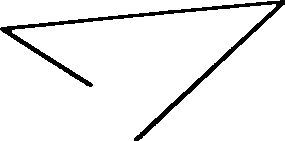
\includegraphics[width=0.75\textwidth]{figures/quad1.png}
	\end{subfigure}
	\begin{subfigure}{0.5\textwidth}
		\centering
		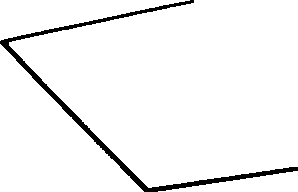
\includegraphics[width=0.75\textwidth]{figures/quad2.png}
	\end{subfigure}
	\caption{Example for different quads}
	\label{fig:exampleQuads}
\end{figure}

%-----------------------------------------------------------------------------------------------
\section{RQIM}
%-----------------------------------------------------------------------------------------------

%-----------------------------------------------------------------------------------------------
\chapter{Quad detection}\label{sect:quad_detection}
%-----------------------------------------------------------------------------------------------

In this chapter there will be a summary of the image processing algorithms tried and used for the recognition of the fiducial markers.
From a computer vision point of view the task is to detect joint line segments.
This is a well researched task in image processing, there are many well tried algorithms for it.

In this chapter will be a short summary of the algorithms used for testing and performance comparison.


The general flow of processing is the same for every line fitting solution.


The process here diverges depending on which line fitting algorithm is used.
They all need differently conditioned input images for optimal performance.
The line fitter routines not necessarily have the same output format\footnote{Some return line segments defined by their endpoint, others use the polar representation of a line etc.}, so conversion may be needed.
This is the end of the marker recognition phase.
This step of the process takes the raw input image and initiates quad structures based on the observed picture.

Three separate line fitting techniques and their variants were profiled in this experiment.
\begin{itemize}
	\item Hough-transformation
	\item Corner detection
	\item Line Segment Detector\cite{LSDDet}
\end{itemize}
The first one uses the Hough-transformation for line detection.
There are many variants of the transformation: Standard Hough Transform, Probabilistic Hough Transform, Multiscale Hough Transform, etc...
The 2 most commonly used are the standard- and the probabilistic variants.
The OpenCV framework offers implementations for them, both were tested in the experiment.

The second detector is based on corner recognition.
There are more variants of this method to try out, too.
The corner metrics of a feature can be calculated differently with (Harris metric, eigenvalues, etc.) varying results.
It is also needed for the solution to be scale invariant, which also can be achieved in a number of ways.

The third alternative is the Line Segment Detector algorithm described in \cite{LSDDet}.
It is a robust and fast algorithm for detecting line segments on an image.
The OpenCV framework provides an implementation of it as well.

A typical marker shot with partial visibility is shown figure \figref{partialMarkerShot}.
\begin{figure}[ht]
	\centering
	
\includegraphics[width=0.75\textwidth]{figures/t35_01.JPG}
	\caption{Partially visible marker (taken with commercial smartphone)}
	\label{fig:partialMarkerShot}
\end{figure}


%-----------------------------------------------------------------------------------------------
\section{Theoretical Overview}
%-----------------------------------------------------------------------------------------------

%-----------------------------------------------------------------------------------------------
\subsection{Hough transformation}
%-----------------------------------------------------------------------------------------------

One of the most commonly used methods for line detection on images is the Hough transform.
Over it's long history many publications have been made about it's applications, performance and improvements.

Originally it was developed by Paul Hough in 1959 and later patented in 1962\cite{houghPatent}.
It was intended to be used for machine analysis of bubble chamber photographs.
In it's modern form (with the $\theta-\rho$ parametrisation) was introduced in 1972 by Duda and Hart\cite{houghThetaRho}.
The transformation became popular in the image processing community after Ballard's article\cite{BALLARD1981111} about generalising the algorithm for detection of arbitrary shapes.
There were many optimised and improved variants of the transformation, however the basic concept remained the same.
In 1990 a publication\cite{XU1990331} introduced the Randomized Hough Transform, which was a fundamentally new approach to the algorithm with notable merits.
As opposed to the one-to-many mapping of the simple Hough transform, the randomised version uses a convergent many-to-one mapping when creating the parameter space.

In this work the Standard Hough Transform and one of it's optimised versions, the Progressive Probabilistic Hough Transform will be used.
The PPHT, although being probabilistic, doesn't belong to the class of randomised Hough transforms.
It uses the same one-to-many mapping as the SHT.
The OpenCV framework provides implementations for the SHT and the PPHT, which is one of the main reason why they were chosen for this project.

After this short historical overview the theory of the transformations will be discussed.

%-----------------------------------------------------------------------------------------------
\subsubsection{Standard Hough Transform}
%-----------------------------------------------------------------------------------------------

The transformation is used to find instances of a model on digital images.
The models are usually simple geometric shapes like lines, circles or ellipses.
The curves are described by their parameters, e.g. slope and intercept for a line, centre point and radius for a circle etc..
Every non-zero pixel\footnote{The transformation works on binary images} votes for the features it could be part of.
The number of votes is stored for every possible parameter combination.
Then a threshold is applied to the stored votes, and the remaining parameters are accepted as model instances.
	
At first Hough described the algorithm to lines, but later the method would be generalised to any analytic\footnote{The Generalised Hough Transform even extends to arbitrary shapes} curve or shape.
This theoretical overview is based on the example of line detection.
The process is the same for every analytic curve, the only difference is the parameter space's dimension.
The original patent\cite{houghPatent} used the slope-intercept representation of lines.
\begin{equation}
y = m*x + b
\end{equation}
In this case, the \emph{parameter space} is 2 dimensional and it's axes are $m$ and $b$.
Every point in the parameter space represent an image space line.
With this representation every non-zero pixel in the image space transforms into a line in the parameter space.
For a given $(x_0,y_0)$ pair \eqref{houghLineMB} gives the line in the parameter space. 
\begin{equation}
\label{eq:houghLineMB}
b = -x_0*m + y_0
\end{equation}
Collinear points in the image show up in the parameter space as intersecting lines.
The more lines intersect in a given $(m_0,b_0)$, the more likely it is the image contains the $y = m_0*x + b_0$ line.
The problem with this parametrisation is that the parameter space is unbounded along both axes.
Both intersect and slope can have values in the range of $(-\infty, \infty)$.
Duda and Hart\cite{houghThetaRho} proposed an alternative parametrisation, which turned out to be better for application.
They used the \emph{normal parametrisation} of a line, shown in \eqref{normalParams}.
\begin{equation}
	\label{eq:normalParams}
	\rho = x*cos(\theta) + y*sin(\theta)
\end{equation}
In \eqref{normalParams} $\rho$ means the distance of the line from the image plane's origin.
$\theta$ is angle of the normal vector of the line.
\begin{figure}[ht]
	\centering
	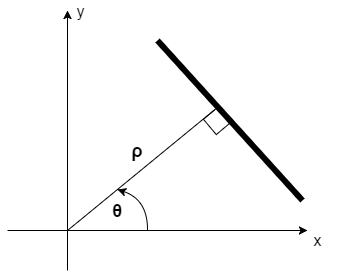
\includegraphics[width=0.5\textwidth]{figures/line_params.png}
	\caption{Normal line parameters}
	\label{fig:normalLineParams}
\end{figure}
If the \emph{normal parametrisation} is used the parameter space becomes finite in both dimensions.
$\theta$ is in the range of $(0,2\pi)$, $\rho$ is bounded by the image size.
In this case the image points define sinusoid curves in the parameter plane, and the line detection is done by searching for their intersections.
\begin{figure}[ht]
	\centering
	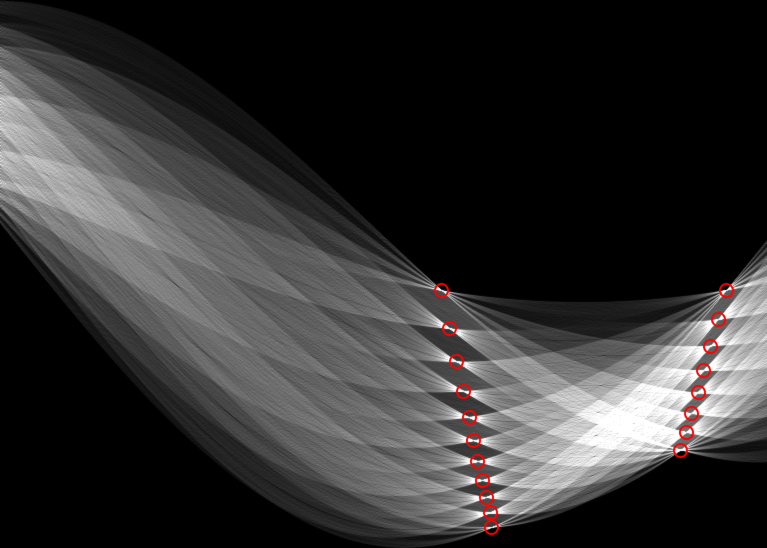
\includegraphics[width=0.6\textwidth]{figures/Perspective_chessboard_hough_transform.png}
	\caption{Hough-transform of a chessboard pattern}
	\label{fig:houghChessBoard}
\end{figure}

As mentioned before, the line detection is based on a voting scheme.
The parameter space (in this case a 2 dimensional plane) is divided into \emph{bins}.
$\rho$ and $\theta$ are quantised in the desired resolution.
The discrete $(\rho,\theta)$ pairs define the bins.
Every bin has accumulator.
When a given $(\rho_i,\theta_i)$ pair gets a vote it's corresponding accumulator is incremented by 1.
The \textbf{SHT} (Standard Hough Transform) uses one-to-many divergent mapping.
This means that every non-zero pixel votes for every possible parameter pair it could belong to.
The above mentioned sinusoid is calculated with the desired resolution for the pixel, and the corresponding accumulators are updated.

When the accumulation phase is completed for the whole image, the local maxima of the accumulators are found.
Usually a threshold is applied in order to reduce noise and eliminate too short line segments.
The radius of the non-maxima suppression also has impact on the results of the line fitting, it must be chosen carefully.
After this step the parameters for the most likely line candidates are available.

As the \textbf{SHT} does not provide the endpoints of the line, they must be found by examining the original binary image.
This can be done by simple checking every pixel along the line with the given parameters and deciding whether or not it is part of the feature.
If it is desired, lines with gaps can also be accepted with this method.
For more accurate fitting, a Least Squares approximation can also be applied to the pixels belonging to the line.

%-----------------------------------------------------------------------------------------------
\subsubsection{Progressive Probabilistic Hough Transform}
%-----------------------------------------------------------------------------------------------

The progressive probabilistic Hough transform is an optimised version of the SHT described in \cite{MATAS2000119}.
Probabilistic Hough transform variants were developed to overcome the comparatively high computational cost of the standard transform.
The core concept is the same for most probabilistic versions of the Hough transform: not every none-zero point votes, only a randomly selected subset.
These algorithms have to find a balance between minimising the proportion of image points that are used for voting while maintaining the accuracy of the detection process.

The original probabilistic Hough transform\cite{KIRYATI1991303} solved this issue by introducing a tunable parameter $p$ for the fraction of points to be used.
First, a $p$ fraction of the non-zero points are selected, than the SHT is performed on the selected subset.
$p$ can be low, the authors of \cite{KIRYATI1991303} presented successful experiments with $p=2\%$.
However, the results of the algorithm are greatly sensitive to the sampling rate.
The authors analysed the problem on the special case of a single line immersed in noise and tried to formulate a solution for determining the $p$ parameter.
They succeeded, but the practical applicability is severely limited\cite{MATAS2000119}: it requires \textit{a priori} knowledge of the number of points belonging to the line.
There was another approach to calculate the number of necessary votes\cite{BERGEN1991639}.
It was shown that the probabilistic Hough transform can be formulated as the Monte Carlo approximation of the SHT, thus it is possible to deduce the desired error rate using the theory of Monte Carlo evaluation.
Nevertheless, the core problem remained the same: \textit{a priori} information was necessary for determining the sampling rate parameter.
Usually there is only very limited information available, so conservative approximation is needed.
This leads to the calculation of more votes then necessary, thus reducing the main advantage of the probabilistic method.

The progressive probabilistic Hough transform solves the above issue by \textquote{exploiting the difference in the fraction of votes needed to reliably detect lines (features) with different number of supporting points}\cite{MATAS2000119}.
This way for long lines only a small fraction of the line's points have to vote for the line to be registered.
For shorter lines this proportion is of course higher.
For lines with supporting points close to the votes generated by background noise a full transform must be performed.

The authors of \cite{MATAS2000119} proposed the following algorithm to achieve the aforementioned goal.
At each iteration a random non-zero image point is selected for voting to the possible model instances it could belong to.
After each vote, the question \textquote{could the count be due to random noise?}\cite{MATAS2000119} is evaluated.
This requires a single comparison per bin update, with a threshold value changing by each vote cast.
When a model instance (line) is detected, the supporting points retract their votes.
The other points belonging to the same line are removed from the voting process.
The pseudo-code representation below is directly quoted from \cite{MATAS2000119}.

\begin{lstlisting}
1. Check input image, if it is empty then finish
2. Update the accumulator with a single pixel randomly selected from the 
   input image
3. Remove pixel from input image
4. Check if the highest peak in the accumulator that was modified by the 
   new pixel is higher than threshold l. If not then goto 1.
5. Look along a corridor specified by the peak in the accumulator, and find 
   the longest segment of pixels either continuous or exhibiting a gap not 
   exceeding a given threshold.
6. Remove the pixels in the segment from the input image
7. Unvote from the accumulator all the pixels from the line that have 
   previously voted.
8. If the line segment is longer than the minimum length add it into the 
   output list.
9. goto 1.
\end{lstlisting}

This algorithm has some considerable advantages of the standard and other, previous probabilistic variants of the Hough transform.
It eliminates the need of \textit{a priori} knowledge necessary for the tuning of probabilistic transforms while it remains much faster than the SHT.
It should detect every instance of a model detectable by the SHT, at the latest when the voting finishes with the same number of voted pixels as for the standard transform.
Another positive property of the algorithm is that features are detected as soon as the accumulator allows a decision: it is not necessary for all supporting points to vote.
The algorithm can also be terminated at any time and still provide some useful output\footnote{However this aspect is not really important for this project}.

Originally this transformation method was developed to speed up the Hough transform, while not being considerably more inaccurate.
However, an unexpected result was observed by the authors.
The PPHT outperformed the SHT in accuracy as well as speed.
In sample images consisting of randomly positioned equal length lines, the PPHT produced less false negatives (missed line segments) and less false positives (incorrectly detected lines).
This effect is due to the fact that PPHT clears out the votes of the detected lines as soon as they are found.
This reduces the clutter in the accumulator, resulting in more accurate results, while also being more computationally efficient.

It also worth noting that the PPHT could, in theory, use every enhancement that were developed for the SHT.
For example, the image gradient of the line segments could be used to reduce the number of pixels selected for voting.
However, this aspect was not researched in the boundaries of this project.

%-----------------------------------------------------------------------------------------------
\subsection{Line Segment Detector}
%-----------------------------------------------------------------------------------------------

%-----------------------------------------------------------------------------------------------
\subsection{Corner Detection}
%-----------------------------------------------------------------------------------------------

Detecting quads not necessarily means the detection of line segments.
Along with the above described methods based on line detection, a corner detecting algorithm was also benchmarked.
The concept of this detection method is as follows.
Detect the corners and end-points of a quad with some corner detection algorithm.
Checks which detected pairs are connected with lines (or edges).
Based on the connected pairs and their ordering, a quad can be reconstructed.

The OpenCV framework provides implementations for some popular corner detection algorithms.
Specifically the Harris detector and the Shi-Thomas detector are covered.
In this section will be a short theoretical summary of corner detection in general, and some specifics of the above mentioned solutions.

The basic idea of most corner detection algorithm is the following.
Considering a local window on an image, corner regions show large change in average intensity if the window is shifted by a small amount in any direction.
The mathematical formulation of the following idea is shown in \eqref{moravec}.
$E_{x,y}$ is the change in intensity produced by shifting the window by $(x,y)$.
$I_{u,v}$ is the intensity of the image at the point $(u,v)$, and $w_{u,v}$ specifies the image window.
In the simplest case, the image window is rectangular and it is unity in a specified region and zero otherwise.

% Moravec corner measure
\begin{equation}
	E_{x,y} = \sum_{u,v} w_{u,v} | I_{x+u,y+v}-I_{u,v} |^2
	\label{eq:moravec}
\end{equation}

A naive approach of corner detection is to use \eqref{moravec} as it is.
The local maxima of the minimum of \eqref{moravec} above a certain threshold can be used for a metric.
With this method, three cases have to be considered:
\begin{enumerate}
	\item \textbf{Flat region:} The windowed image region has almost constant intensity. In that case, all shifts will show small change.
	\item \textbf{Edge region:} The windowed image region has an edge in it. In that case shift in one direction will result in large change, but shifts in other directions will show low change in intensity.
	\item \textbf{Corner region:} If the windowed region contains a corner, all shifts will show large change in the intensity.
\end{enumerate}

The shifts can be chosen in a couple of ways: $90^\circ$ shifts, $45^\circ$ shifts in 8 or 4 directions, etc...
Actually, this detection method is analysed in \cite{Harris88alvey}, and it is the base of the Harris detector.

\begin{figure}[ht]
	\centering
	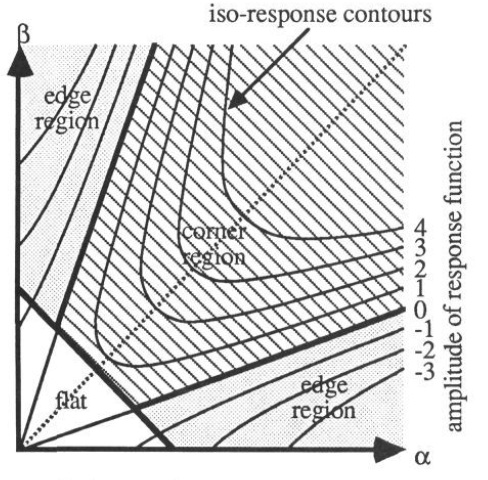
\includegraphics[width=0.75\textwidth]{figures/score-isoresponse-contours.jpg}
	\caption{Image point classification based on Harris measure\cite{Harris88alvey}}
	\label{fig:harrisMeasure}
\end{figure}

However, the the above described corner detector suffers from a number of problems\cite{Harris88alvey}.
Firstly, it provides an anisotropic response, as only a discrete set of shifts are used.
To address this issue, the Harris detector uses an analytic expansion of \eqref{moravec} around origin.
See \eqref{analyticHarris}.
\begin{equation}
	E_{x,y} = \sum_{u,v} w_{u,v} ( I_{x+u,y+v}-I_{u,v} )^2 = \sum_{u,v} w_{u,v} ( x \frac{\partial I}{\partial x} + y \frac{\partial I}{\partial y} + O(x^2,y^2))^2
	\label{eq:analyticHarris}
\end{equation}
Another problem is that the above detection method's response is noisy\cite{Harris88alvey} because of the rectangular and binary image window.
The Harris detector resolves this issue by using a circular and smooth (for example Gaussian) window:
\begin{equation}
	w_{u,v} = e^{- \frac{u^2 + v^2}{2\sigma^2}}
\end{equation}
The third issue Harris found with the use of \eqref{moravec} as a corner metric is that it responds too readily t edges\cite{Harris88alvey}.
This is because only the minimum of $E$ is taken into account when deciding whether a sampled window contains a corner or not.
To address this issue, a reformulation of the corner measure was proposed that takes the variation of $E$ with the direction of the change into consideration.
For small changes, $E$, the average change in intensity generated by a shift with $(x,y)$ can be written as:
\begin{equation}
	E(x,y) = (x,y) M (x,y)^T
\end{equation}
Where $M$ is composed of the image gradients in the window. \eqref{mMatrix} shows $M$ using the notation of \eqref{mMatrixNotation}
\begin{equation}
	I_x = \frac{\partial I}{\partial x}, I_y = \frac{\partial I}{\partial y}
	\label{eq:mMatrixNotation}
\end{equation}
\begin{equation}
\begin{bmatrix}
	I_x^2 && I_x I_y \\
	I_x I_y && I_y^2
\end{bmatrix}
	\label{eq:mMatrix}
\end{equation}
Note that $M$ describes the shape of the local autocorrelation function's shape at the origin.
To describe $E$, \cite{Harris88alvey} uses the eigenvalues of the matrix $M$, as it provides a rotationally invariant description.
With this new method, the above mentioned cases (flat region, edge, corner) can be expressed as follows.
\begin{enumerate}
	\item \textbf{Flat region:} Both eigenvalues are small.
	\item \textbf{Edge region:} One eigenvalue of $M$ is small, the other is comparatively large.
	\item \textbf{Corner region:} Both eigenvalues are high.
\end{enumerate}
Figure \figref{harrisMeasure} shows the above defined regions with respect to the eigenvalues ($\alpha$ and $\beta$ are the eigenvalues of $M$).
The Harris detector also uses a metric for the "quality" of the detected edges or corners.
This is noted with $R$ and is defined below.
% Harris Measure
\begin{equation}
R = \det(M) - k(Trace(M))^2
\end{equation}

This is the short theoretical summary of the Harris detector.
A detailed mathematical derivation of the formulae can be found in \cite{Harris88alvey}.

\begin{figure}[ht]
	\centering
	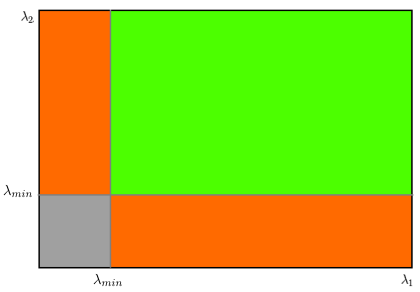
\includegraphics[width=0.75\textwidth]{figures/shitomasi_space.png}
	\caption{Image point classification based on Shi-Tomasi measure. Image source: OpenCV documentation}
	\label{fig:shitomasiMeasure}
\end{figure}

%-----------------------------------------------------------------------------------------------
\section{Application for Quad Detection}
%-----------------------------------------------------------------------------------------------


%-----------------------------------------------------------------------------------------------
\subsection{Conditioning}
%-----------------------------------------------------------------------------------------------

Before running the line detection algorithms some conditioning steps are done in order to improve their effectiveness.
These processes are not uniform - every fitting method needs it's own.

The Hough transformation traditionally works best on thin lines.
The easiest way is to generate an edge image with high-pass filtering.
The OpenCV framework offers a wide variety of features for this task.
The best result are obtained by using the Canny edge detector.

The skeletoning detector does not need a conditioning step, as it performs the band thinning on it's own.

The methods based on image gradients and corner detection both require some level of smoothing on the picture.
In case of the corner detection the smoothing is useful for removing the false positive matches caused by the jagged edges, or in case os JPEG images the artefacts caused by the compression.
The gradient detector simply gives a more spread-out and easier to analyse result on a smoothly changing gradient than it would on strict edge.
The smoothing is also implemented using the OpenCV framework, which provides easy access to Gaussian filtering.
The OpenCV implementation is based on convolution with a configurable Gaussian kernel.
The kernel size and the deviation in $x$ and $y$ direction can be set.
The Gaussian kernel and the convolution itself is handled in the framework.



%-----------------------------------------------------------------------------------------------
\chapter{Marker-based Pose Estimation}\label{sect:marker_recognition}
%-----------------------------------------------------------------------------------------------

The main goal fo this work is to devise a fiducial marker and a method of estimating the camera pose based on it.
In the previous chapters the most of the building blocks used to achieve this were laid out.
The marker have been defined and the image processing algorithms used for measuring quad positions were explained.
In this chapter a solution will be given to the task of estimating the camera pose based on a single shot of the above described markers.

\begin{figure}[ht]
	\centering
	
\includegraphics[width=0.9\textwidth]{figures/marker_full.JPG}
	\caption{Shot of a partially visible marker covering the whole field of vision}
	\label{fig:markerFull}
\end{figure}

As it's input, the algorithm will receive an image containing the marker (figure \figref{markerFull} shows an example).
The image does not have to be ideal.
Quite probably some of the marker's surroundings are also visible, or equally probably only a part of the marker is visible.
Using commercially available cameras the image almost certainly contains some level of noise.
The algorithm has to be prepared for handling these cases.
This is achieved by applying a range of preprocessing steps to the input image.

When the input image have been aptly conditioned, the regions containing quads have to be identified.
The previously described quad detection routines work on images containing a single quad\footnote{Although they could be implemented to handle whole markers at once}, so the input have to be segmented before quad detection.
These two steps (identifying quad-like regions and segmentation) are done in a single a step based on extracting blobs that meet certain criteria typical for quads.

The next step in the processing pipeline is running the quad detection algorithm on the previously selected segments.
It is executed for each quad-like blob, and the successfully identified quads are stored in a list for later processing.
If enough quads have been found, the pose can be calculated.

The last necessary step is to actually estimate the camera pose.
This is an iterative process, as the pairing of original and detected quads are not known prior to successfully approximating the viewpoint.
This algorithm was designed supposing the marker on the image is known and only the camera pose has to be calculated.
For the purposes of this project the assumptions is reasonable, as for now, no meta-information is coded into the markers.
Also, for the current stage a single point of reference for the pose is enough.

The above steps of the pose estimation algorithm are summarised in the following pseudo-code.
\begin{lstlisting}
estimate_pose(img, original_marker):
    img = prepare_img(img)
    quad_imgs = get_segments(img)
    quads = empty_list
    for quad_img in quad_imgs
        quad = detect_quad(quad_img)
        quads.append(quad)
    pose = find_pose(quads, orignal_marker) 
    return pose
\end{lstlisting}
The following sections will elaborate on each step of the process.
The quad detection algorithms were already covered, their explanation can be found in the relevant chapter.
The pose calculation from the corresponding point pairs will also not be covered, as the algorithm was described in chapter 1.

%-----------------------------------------------------------------------------------------------
\section{Preprocessing}
%-----------------------------------------------------------------------------------------------

The input of the preprocessing step is the raw image taken\footnote{In the development phase rendered pictures were used for better repeatability} by the observer.
The goal of this step is preparing the input image for the next phases (segmentation, filtering, quad detection) of processing visual data.
As mentioned in the introduction, the raw input image can have a variety of distortions.
Some of these are systematic and thus easy accounted for, others are random and their effects can only be dampened.
An example of the first one the barrel distortion caused by the camera lens, and of the latter is the \textit{salt and pepper} noise of the image.

The systematic errors are corrected by using a calibrated camera.
Camera calibration will not be covered in depth, as multiple well tried solutions exist for it.
In this project a calibration method provided by the OpenCV framework was used.
It uses a chessboard pattern as a calibration image to measure the intrinsic camera parameters.
The OpenCV framework uses \eqref{cameraMat} for a camera model.
\begin{equation}
	C_m = 
	\begin{bmatrix}
		f_x & 0   & c_x \\
		0   & f_y & c_y \\
		0   & 0   & 1
	\end{bmatrix}
	\label{eq:cameraMat}
\end{equation}
The parameters correspond to the usual notation:
\begin{itemize}
	\item $f_x, f_y$: Focal lengths of the camera in $x$ and $y$ direction
	\item $c_x, c_y$: The coordinates of the optical centre in the image
\end{itemize}
Based on the camera matrix, OpenCV can account for most of the radial and tangential distortion in the image.

The filtering of random noise from the image is a bigger issue, and no exact solution can be given for it.
There are many factors that can influence the quality of the image.
The lighting conditions, the shadows, the viewing angle, etc...
Not all of them can (reasonably) be accounted for.
However, to lessen their impact on the image, the following steps are taken.

First the photos are converted to binary format by applying a threshold.
The image is inverted in the process, because it makes more sense for the objects to be marked with non-zero elements than vice-versa.
The threshold's value is determined using Otsu's method, which maximises the inter-class variance of the clusters\footnote{Foreground and background}.
The implementation is provided by the OpenCV framework.

Afterwards, the binary image is conditioned with a \emph{close} morphology operator.
The closing removes the gaps from the large connected areas (possible quads) and removes the \emph{salt and pepper}-like noise.
In the current implementation the kernel size of the morphology operator is constant, however it could be beneficial to calculate it from the global or local image parameters\footnote{e.g. image size, area of the connected region, etc.}.

\begin{figure}[ht]
	\centering
	
\includegraphics[width=0.9\textwidth]{figures/marker_full_preprocessed.JPG}
	\caption{Marker image after preprocessing}
	\label{fig:markerFullPreproc}
\end{figure}
Figure \figref{markerFullPreproc} shows the output of the preprocessing step of the algorithm.
This is passed to the segmentation logic described in the next section.

%-----------------------------------------------------------------------------------------------
\section{Segmentation}
%-----------------------------------------------------------------------------------------------

The segmentation process is carried out on images roughly like the one shown in figure \figref{markerFullPreproc}.
The segmentation is based on finding continuous contours on the binary image.
The OpenCV framework provides great functionality for this.
The implementation is based on calculating the 8-neighbour chain code for the binary blobs on the image.
The functions returns a list of points for the borders of each distinct contour.
These can be used for calculating the area and circumference of the blobs represented by the contours.

The next step is the filtering of the found blobs.
First, it is necessary to discard the only partially visible and/or unrecognisable quads.
This is done by calculating the bounding box of the contours, and if one of it's sides are touching the image border, the blob is marked as partial.
With this approach it is possible that some fully visible quads that only touch the image border with one of their corner are lost.
This problem can be easily fixed by checking the neighbourhood of the contact point, but this is not yet implemented.

\begin{figure}[ht]
	\begin{subfigure}{0.3\textwidth}
		\centering
		
\includegraphics{figures/quad3.png}
	\end{subfigure}
	\begin{subfigure}{0.3\textwidth}
		\centering
		
\includegraphics{figures/quad4.png}
	\end{subfigure}
	\begin{subfigure}{0.3\textwidth}
		\centering
		
\includegraphics{figures/quad5.png}
	\end{subfigure}
	\caption{Quad candidates after segmentation}
	\label{fig:segmentationOutput}
\end{figure}

The next blob-filtering step is to filter out the false-positive contours.
These false hits can be caused by the light conditions or the scene around the marker.
For this purpose a simple metric is used to measure how likely a blob is to be a quad. 
This metric is the ratio of a blob's area and circumference. 
By experimentation this ratio for quads is found to be in the range of 10 and 50.
The contours with ratios outside these limits are discarded.

The segmentation processes output is available as a singe image with colour-coded\footnote{Gray level, to be exact} blobs or as a list of separate images each containing a quad candidate.
At the current state of the project only the image list representation is used, as te implemented quad detectors take images of single quads as their input.
However, the possibility of implementing detectors to work on whole RQIMs is left open by the colour-coded representation.
Figure \figref{segmentationOutput} shows an example for the output of the segmentation process.

There is also the problem of finding the RQIM on the picture.
This topic was not thoroughly researched in this work, but some basic guidelines were brought up.
The above described segmentation process can be used to identify a marker.
By running the segmentation and filtering process the density of probable quads per image region can be calculated.
On a marker, this should be above the noise level.
By using \textit{a-priori} knowledge of the approximate marker size, the RQIM region on the image can be identified.
When this region is selected, the found probable quads outside it can be discarded.

At this point there is an image or set of images containing potentially good quads.
These are passed as input to the quad detector.
After the quad detection, all image processing tasks are complete.
From then on, only the quad representations are used.

%-----------------------------------------------------------------------------------------------
\section{Pose Calculation}
%-----------------------------------------------------------------------------------------------

The last step of the algorithm is to actually calculate the pose from the detected quads.
According to chapter \sectref{pose}, this is done by using the \textit{robust pose estimation from a planar target} algorithm.
However, the association between the original and the detected quads is not known.
The quad coordinates measured in the previous processing step are of the quads distorted by the projection.
At first, this looks like a deadlock situation: the association of the quads is needed to calculate the camera pose, but without the pose the quads cannot be paired.

To resolve the above issue, an iterative process is proposed.
It is summarised by the following pseudo-code.
The method is a variant of the Random Sample Consensus algorithm.
It's core concept is that randomly selected quad pairs are tested, and the one having the highest number of inliers and least error level is accepted as a solution.
\begin{lstlisting}
find_pose(det_quads, orig_quads):
    threshold = get_thresh(count(det_quads), count(orig_quads))
    pairs = combinations(det_quads, orig_quads)
    pairs.shuffle()
    best_pose = none
    best_error = inf
    for det, orig in pairs:
        pose = robust_planar_pose(det, orig)
        matches = test_pose(pose, det_quads, orig_quads)
        if count(matches) > threshold:
            error = get_detection_error(matches)
            if error < precision:
                return pose
            else if error < best_error:
                best_pose = pose
                best_error = error
    return pose
\end{lstlisting}



%%-----------------------------------------------------------------------------------------------
\chapter{Conclusion}\label{sect:conclusion}
%-----------------------------------------------------------------------------------------------

During the course of this work the process of calculating camera pose was thoroughly examined.
Each step from getting the input image to calculating the camera pose was discussed.
For most parts both the underlying theory and empirical test results were presented.

In line with the project targets, multiple pose estimation methods were discussed and compared.
The EP$n$P\cite{Lepetit2008}, an iterative approach\cite{iterative} and the robust pose estimation\cite{robust} were considered as candidates to be used in this project.
Short summaries of their operating principles were presented.
Their performance then was compared with respect to multiple properties: accuracy, robustness, and computational efficiency.
As a result, two algorithms were selected depending on the available computational power available on the target platform.
EP$n$P is recommended for use on mobile devices or embedded platforms, where efficient, non-iterative solution is preferred.
However, if robust and accurate results are necessary (and there are enough resources), the robust pose estimation algorithm is the better choice.

Another focus of the project was developing a marker with advantageous properties for pose estimation.
To achieve this goal the RQIM was proposed.
It is a randomly generated marker put together from multiple quads.
It has been shown to have desirable properties for pose estimation: scale invariance and redundancy.
A formal representation of the quads (both mathematical and computational) have been defined.
A simple algorithm was proposed for generating random markers.
The notion of creating discrete parameter space for quads has also been examined.
It would provide additional robustness and the ability to encode meta-information in the markers, however these possibilities have not been tested.

The main part of this work is dedicated to the development and testing of a marker detecting solution.
It was shown that marker detection is (from an image processing point of view) equivalent to detecting individual quads on the source image.
Two different approaches were made to quad detection: line detection-, and corner detection based solution.
Multiple line detection algorithms were considered for use.
To make a more informed decision on which one to use, their theoretical foundations have been summarised.
The theory of corner detection was also covered.
Four different quad detectors were developed and tested: each based on a different underlying algorithm.
Their implementation details were discussed and their python source code is published in the appendix.

The quad detectors were not only compared based on the theoretical capabilities of their underlying algorithm, they were also extensively tested.
A testing methodology have been developed for comparing the algorithms.
The test were run on randomly generated quads with fixed sizes.
For each size, a 1000 instance was generated to guarantee that the results are statistically significant.
To quantify the detection error, multiple error functions were defined.
The detectors were compared by the ones that describe the overall error in detection.
Error functions were defined for each quad parameter; with their help, the distribution of inaccuracy between the parameters were examined.

Based on the data obtained by the tests, the LSD\cite{LSDDet} line detector based implementation was selected.
It proved to be the most accurate and resistant to noise.
It is also an efficient algorithm that runs in linear time.

The final part of this work was about organising the above components into a complete pose estimation solution.
Images used as input for pose estimation have to be preprocessed and filtered for noise.
These steps of the processing pipeline have been described in chapter 4.
The detected quad structures of a marker are used as input for the pose estimation algorithms selected in chapter 1.
A RANSAC-like approach was proposed for finding the correspondences between the detected and the original quads.
%\listoffigures\addcontentsline{toc}{chapter}{Ábrák jegyzéke}
%\listoftables\addcontentsline{toc}{chapter}{Táblázatok jegyzéke}

\bibliography{mybib}
\addcontentsline{toc}{chapter}{Bibliography}
\bibliographystyle{plain}

%----------------------------------------------------------------------------
\appendix
%----------------------------------------------------------------------------
\chapter*{Appendix}\addcontentsline{toc}{chapter}{Appendix}
\setcounter{chapter}{1}  % a fofejezet-szamlalo az angol ABC 6. betuje (F) lesz
\setcounter{equation}{0} % a fofejezet-szamlalo az angol ABC 6. betuje (F) lesz
\numberwithin{equation}{section}
\numberwithin{figure}{section}
\numberwithin{lstlisting}{section}
%\numberwithin{tabular}{section}


\label{page:last}
\end{document}